\scanpage{350}
\mspage{89}
% archive sheet number: 349
Ceci vu, l'idée naturelle pour ``déformer'' $F$ en $F_0$, c'est de trouver une suite d'homotopies qui transforment $F$ de façon à lui faire acquérir successivement les caractéristiques a), b), c) du voyageur pressé. \deleted{Pour} Au besoin, pour aller plus vite au but, on utilisera l'hypothèse de récurrence sur \deleted{\unsure{$n$}} \inserted{$n=\mathrm{long.}\,\tau$}, que le théorème \deleted{\unsure{est pr}} de connexité est \inserted{déjà} prouvé quand $I_{\unsure{\tau}}$ est de longueur \deleted{utile} $\leq n-1$. (NB Le \deleted{\unsure{est}} th. est trivial pour $\unsure{N|n|\tau}\leq1$, car alors les cat. $\underline{\mathrm{Hom}}_{\unsure{\varepsilon}}(\tau,\tau')$ sont \inserted{toutes ou bien} vides, ou bien ponctuelles)

\deleted{\unsure{Plusieurs} \deleted{\unsure{en}} étapes}

\deleted{1) Supposons qu'il y ait deux flèches \deleted{\unsure{de}} $F$-critique\unsure{s} consécutives \inserted{(dans la suite tot. ordonnée des fl. $F$-cr.)} de même signature, \deleted{\unsure{soient donc} $\underline{u}_k$ et $\underline{u}_\ell$ $(k<\ell)$, on va donc, par une suite de déformations, \unsure{désignons}} de $F$, qui \unsure{ne bougeront|en bougeant} $F$ \deleted{\unsure{pour}} sur les intervalles critiques $I_{k'},I_{\ell'}$ ($k'\leq\ell'$) qui contiennent $\underline{u}_k,\underline{u}_\ell$, et sur les éventuels \unsure{int. cr.} intermédiaires (si $k'<\ell'$), \deleted{mais pas sur les autres intervalles critiques, \unsure{coll}} Groupons ensemble toutes les flèches de tr. critiques d'une $=$ \deleted{\unsure{groupe de t}} \inserted{suite} maximale}
\deleted{\[
\deleted{\unsure{\underline{u}_{k},\underline{u}_{k+1},\ldots,\underline{u}_{k+t}}}
\inserted{\underline{u}_{i_\alpha},\underline{u}_{i_{\alpha+1}},\ldots,\underline{u}_{i_{\alpha+t}}}
\]}
\deleted{de \inserted{$t+1$} flèches critiques consécutives de $=$ signe $\varepsilon$ \unsure{(Et ex)|(Et soit}, c'est-à-dire que si $\alpha>1$, $\underline{u}_{i_{\alpha-1}}$ est de \deleted{\unsure{même signe que} $\varepsilon$,} \inserted{signe $-\varepsilon$,} et de $=$ si $\alpha+t<r'$, $\underline{u}_{i_{\alpha+t+1}}$ de signe $-\varepsilon$. \deleted{\unsure{Alors}} En regardant $p=\mathrm{source}\,\underline{u}_{i_\alpha}$, $q=\mathrm{but}\,\underline{u}_{i_{\alpha+t}}$, et le \unsure{sous-intervalle} $I=[p,q]$ de $I_\tau$, \deleted{\unsure{l'id}} si on \deleted{\unsure{n'a pas}} n'a pas $p=0$, $q=n$ ($=\mathrm{long}\,\tau$), l'hypothèse de récurrence, appliquée à $I$ (avec les signes induits par ceux de $I_\tau$) et à $I'=[f(p),f(q)]\subset I$, nous montre qu'on peut déformer $F$, \unsure{sauf|sans} toucher à}
\margin{$t\geq1$}
% Long tapered ink mark in lower left margin.
\figure{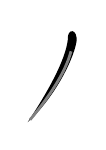
\begin{tikzpicture}[x=1cm,y=1cm]
\fill (0,0) .. controls (.24,.36) and (.48,.78) .. (.51,1.05)
.. controls (.50,1.20) and (.64,1.19) .. (.62,1.02)
.. controls (.57,.75) and (.31,.28) .. (0,0);
\draw[gray,line width=1pt] (.03,.03) .. controls (.24,.28) and (.48,.62) .. (.55,.90);
\end{tikzpicture}}
